\section{Introduction}\label{sec:Intro}
In MR imaging, some tissues have poor \emph{contrast}, which means that the boundaries between tissue types cannot be determined.
 To overcome this, particulate solutions of contrast agent are used to illuminate regions of interest~\cite{na2009inorganic}. 
 Drawbacks include that the contrast agent diffuses quickly and must be injected repeatedly during long scans. 
 Additionally, many contrast agents such as Gadolinium chelates are toxic, and prolonged exposure causes medical complications \cite{caravan1999gadolinium}. 
This paper explores using steerable magnetic micro particles to map a region. 
These particles can be steered by the global magnetic gradient of an MRI and visualised by the MRI \cite{Vartholomeos2012}, even when the tissues they move through  have poor contrast.

As a current example, micro- and nano-particles can be manufactured in large numbers, see~\cite{Chowdhury2015,martel2014computer,kim2015imparting,Donald2013,Ghosh2009,Ou2013,qiu2015magnetic}.

The particles considered in this paper move under the influence of a global command. All particles move in the same direction when commanded. 
In our previous work \cite{mahadev2016collecting} we provided an algorithm that guarantees the collection of particles.
 In this work we explore the field of mapping, coverage, and foraging using globally controlled particles. 
 We assume particle position can be measured, but the workspace cannot be imaged. 
 Particles respond identically to the global input unless they hit an obstacle or another particle. 
 This paper focuses on discrete 2D workspace.
Fig. \ref{fig:Coverage2DwithUnformControl} represents the complete mapping of a workspace with large number of particles.  
At the initial step, all  particles (red circles) are in free cells (white squares) and are surrounded by blue squares that represent the unknown frontier cells.
By commanding the particles to take one step in a particular direction, we can categorize the the frontier cell in this direction as either obstacle or free.
 If the particle was able to move, that frontier cell is labelled as free, and new frontier cells are added to adjacent areas that have not been mapped.
 If the particle was unable to move, that frontier cell is labelled as obstacle.
The goal is to explore all  frontier cells, thereby discovering all connected free cells and the obstacles that surround them. 


The paper is arranged as follows. 
After a review of recent related work in Sec.~\ref{sec:RelatedWork}, we introduce the algorithms to perform the mapping and coverage in Sec.~\ref{sec:theory}.
 Sec.~\ref{sec:simulation} describes implementations of the algorithms in simulation and theoretical validation of efficiency. 
% Sec.  \ref{sec:expResults} 
  We discuss the performance of the algorithms on parameters which determine efficiency and also provide directions for further research in Sec.  \ref{sec:conclusion}.

\begin{figure}
\begin{center}
	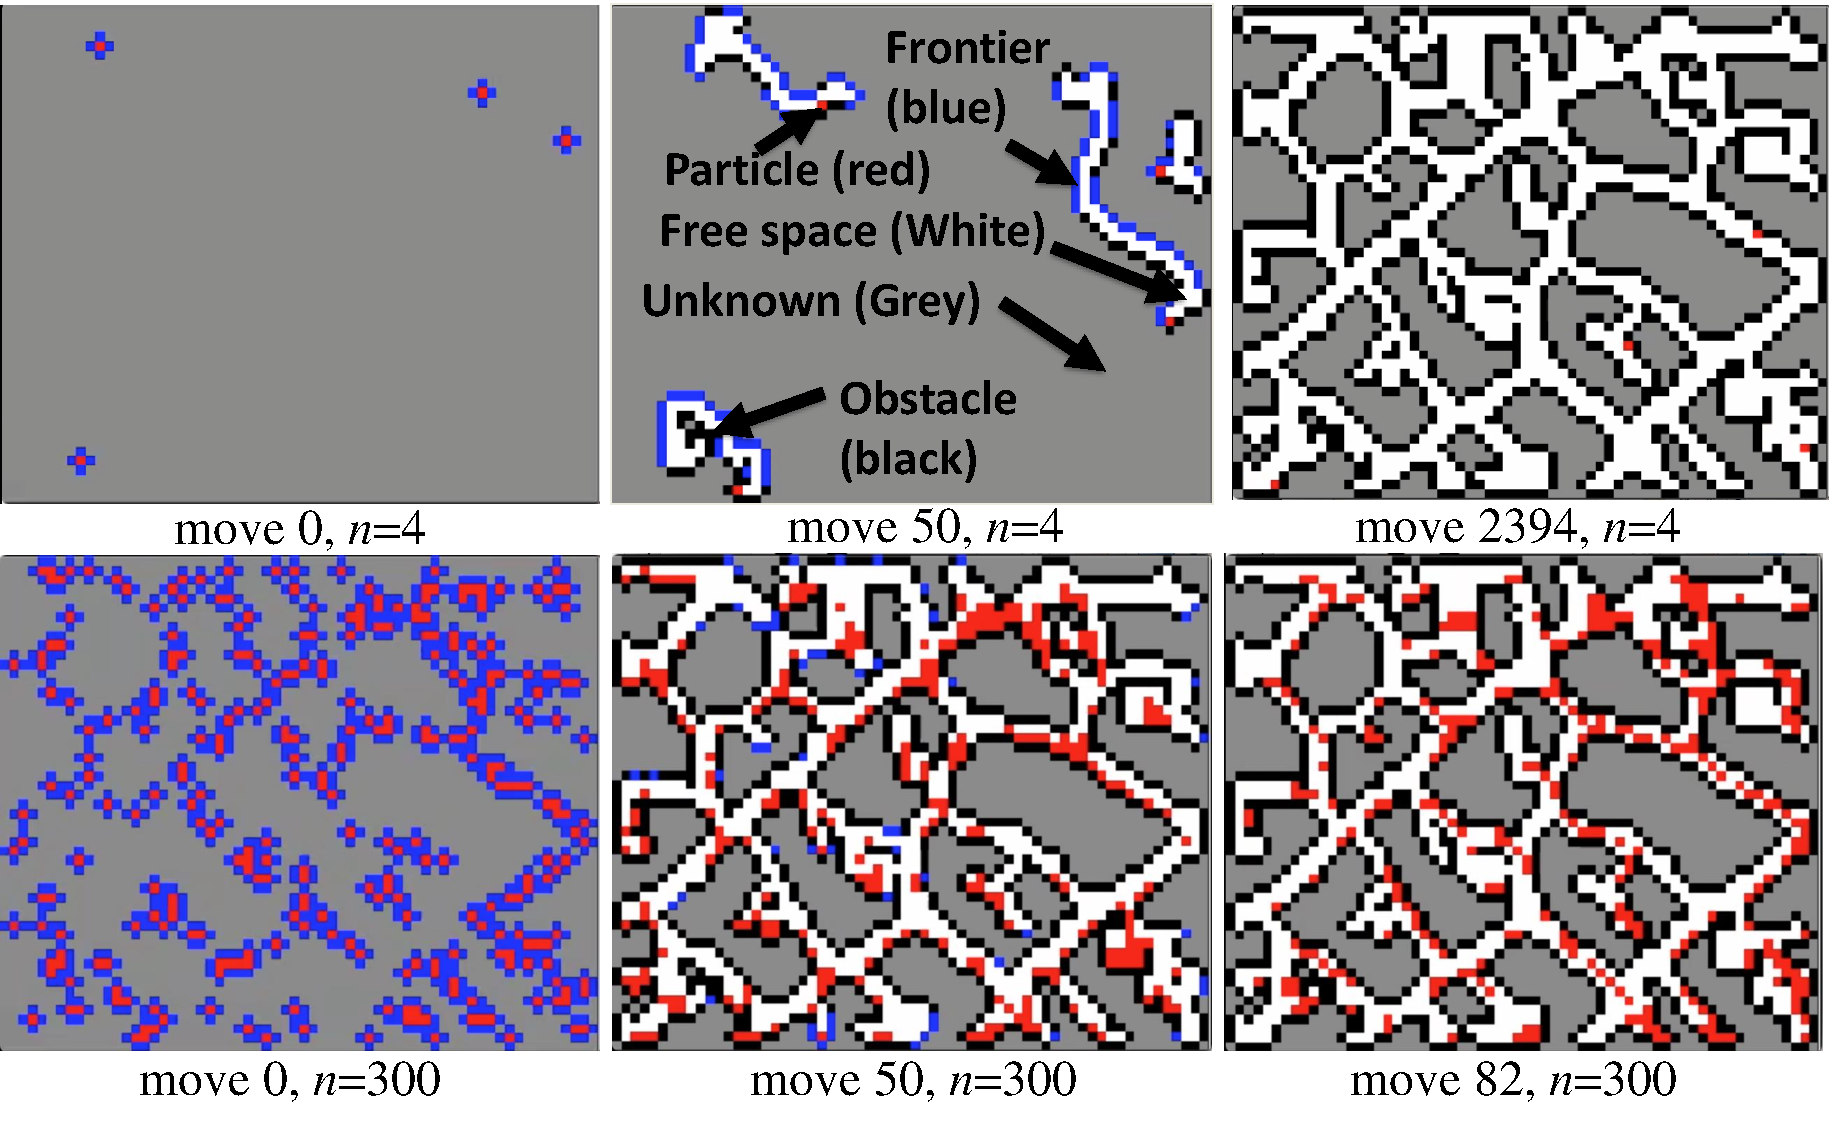
\includegraphics[width=1.0\columnwidth]{Coverage2DwithUnformControl}
\end{center}
\caption{\label{fig:Coverage2DwithUnformControl}
Exploring a 2D environment with 500 blank spaces with $n=4$ (top) and $n=300$ particles, all controlled by a external global force.  After 82 moves, the 300 particles have explored the entire space, while the 4 particles require a total of 2394 moves to fully cover the area. 
}
\end{figure}
